\documentclass{beamer}
\usepackage{svg}
\usepackage{tikz}

\title{Introduction to Machine Learning}
\logo{\includesvg[width=1.2cm]{../NBU}}
\author[Bhaya, A.G.]{Bhaya, A.G.}

\usetikzlibrary{arrows.meta, positioning}
\usetheme{Berkeley}
\usecolortheme{default}

\begin{document}
    \begin{frame}
        \titlepage
    \end{frame}

    \begin{frame}{Table of Contents}
        \tableofcontents
    \end{frame}

    \section{Prerequisites}
    \begin{frame}{Prerequisites}
        \begin{itemize}
            \item Single variable function: \(f(x), f(y)\), etc.
            \item Multivariate functions: \(f(x,y), L(x,w)\), etc.
            \item Linear algebra: matrices
            \item Set theory
        \end{itemize}
    \end{frame}

    \section{Introduction}
    \begin{frame}{Introduction}
        Humans can learn from past experience and make decisions on their own. Consider a baby who identifies different types of vehicle. Based on sufficient learning data, he might be able to differentiate a four-wheeler (car) from a two-wheeler (motorcycle). So, humans can observe and learn from the observed experience.

        We want a similar learning behavior in machines. \textit{``What we want is a machine that can learn from experience.''} --- Alan Turing, 1947.
    \end{frame}

    \subsection{A Simple Example}
    \begin{frame}[allowframebreaks]{A Simple Example}
        \textbf{Example:} Consider the following \(x,y\)-pairs,

        \medskip
        \begin{tabular}{|c||c|c|c|c|}
            \hline
            \(x\) & 1 & 2 & 3 & 4 \\
            \hline
            \(y\) & 1 & 4 & 9 & 16\\
            \hline
        \end{tabular}
        \medskip
        
        Based on the given example, if one were to identify the \(y\)-values for \(x=\{5,6,7\}\), what would the pipeline be?

        Firstly, one would have to find a relationship between the given set of points. If you look closely, the relationship between the \(x,y\)-pair can be defined by \(y=2x\). Now we can apply the defined relationship to the given set of points, \(x:y=\{5:10,6:12,7:14\}\).

        \pagebreak

        This pipeline is exactly the base philosophy behind machine learning. First, we provide \textbf{pre-defined data} (training data), along with the \textbf{ground truth} (\(y\)-values). Secondly, ML defines a relationship between the data points. Finally, we use the defined relationship to create predictions about new unknown data.
     \end{frame}

     \section{What is Machine Learning?}
     \begin{frame}{What is Machine Learning?}
         \begin{figure}
             \centering
             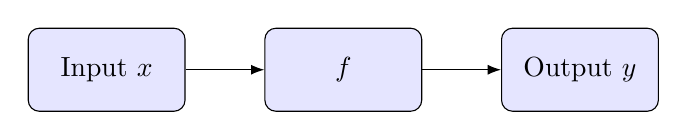
\begin{tikzpicture}[
                    node distance=1cm,
                    block/.style={rectangle, draw, fill=blue!10, text width=5em, text centered, rounded corners, minimum height=3em},
                    line/.style={draw, -Latex}
                ]
                    % Place nodes
                    \node [block] (input) {Input $x$};
                    \node [block, right=of input] (model) {$f$};
                    \node [block, right=of model] (output) {Output $y$};
                
                    % Draw edges
                    \path [line ] (input) -- (model);
                    \path [line] (model) -- (output);
            \end{tikzpicture}
             \caption{Goal of machine learning}
         \end{figure}
         \begin{definition}[Goal of Machine Learning]
             Come up with a rule \(f\) from \textbf{training data} \((x_i,y_i)\).
         \end{definition}
     \end{frame}

     \section{Traditional Programming vs. Machine Learning}
     \begin{frame}[allowframebreaks]{Traditional Programming vs. Machine Learning}
         \begin{figure}
            \centering
            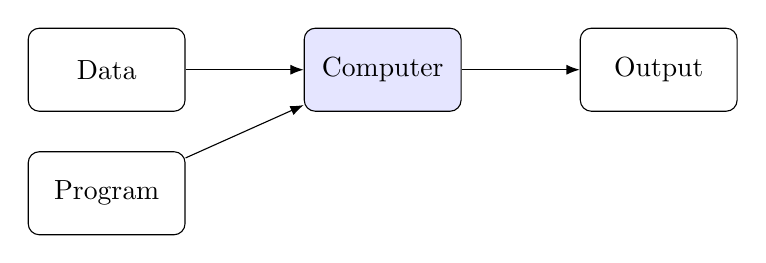
\begin{tikzpicture}[
                node distance=1.5cm, % Increased distance for better clarity
                block/.style={rectangle, draw, fill=blue!10, text width=5em, text centered, rounded corners, minimum height=3em},
                uc_block/.style={rectangle, draw, text width=5em, text centered, rounded corners, minimum height=3em},
                line/.style={draw, -Latex}
            ]
                % Place nodes
                \node [uc_block] (P_data) {Data};
                
                % FIX 1: Use 'below=of' (requires positioning library) instead of 'bottom=of'
                \node [uc_block, below=0.5cm of P_data] (P_prog) {Program}; 
                
                % FIX 2: Added a name (P_prog) to the Program node to anchor lines if needed
                \node [block, right=1.5cm of P_data] (P_computer) {Computer};
                \node [uc_block, right=of P_computer] (P_output) {Output};
            
                % Draw edges
                % FIX 3: Drawing lines from both Data and Program to Computer
                \path [line] (P_data) -- (P_computer);
                \path [line] (P_prog) -- ([yshift=-2mm]P_computer);
                \path [line] (P_computer) -- (P_output);
                
            \end{tikzpicture}
            \caption{Traditional Programming}
        \end{figure}
        
        \begin{figure}
            \centering
            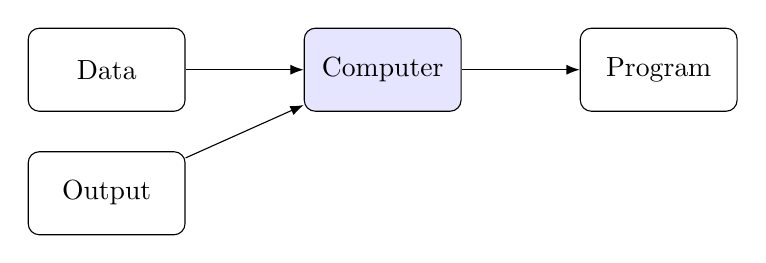
\begin{tikzpicture}[
                node distance=1.5cm, % Increased distance for better clarity
                block/.style={rectangle, draw, fill=blue!10, text width=5em, text centered, rounded corners, minimum height=3em},
                uc_block/.style={rectangle, draw, text width=5em, text centered, rounded corners, minimum height=3em},
                line/.style={draw, -Latex}
            ]
                % Place nodes
                \node [uc_block] (P_data) {Data};
                
                % FIX 1: Use 'below=of' (requires positioning library) instead of 'bottom=of'
                \node [uc_block, below=0.5cm of P_data] (P_prog) {Output}; 
                
                % FIX 2: Added a name (P_prog) to the Program node to anchor lines if needed
                \node [block, right=1.5cm of P_data] (P_computer) {Computer};
                \node [uc_block, right=of P_computer] (P_output) {Program};
            
                % Draw edges
                % FIX 3: Drawing lines from both Data and Program to Computer
                \path [line] (P_data) -- (P_computer);
                \path [line] (P_prog) -- ([yshift=-2mm]P_computer);
                \path [line] (P_computer) -- (P_output);
                
            \end{tikzpicture}
            \caption{Machine Learning}
        \end{figure}
     \end{frame}
\end{document}